\section{Logics}
This section will describe the ''machinery'' behind the simulations. We will
detail how we represent the system (i.e. the bulk or surface) and how we perform
the simulations from a computer science point of view (the physics is discussed
in other parts of this document).
\subsection{The atoms}
Our bulk, or surface, contains a number of individual atoms. Each atom is stored
as a separate instance of an atom class, containing (among other things) the
atom's mass, current velocity, position and acceleration.
\subsection{The Verlet List}
When we run our simulation we crate an array of Verlet Lists (one for each atom
in the bulk), where each entry is a linked list containing all the atoms inside
the verlet skin of the current atom (verlet list i in the list contains atom i
and all it's neighbours). When we update the Verlet Lists we loop through all
atoms in the bulk (or surface) and add all other atoms that are within the
Verlet Skin, in order to avoid double counting the forces acting on each atom we
only add one of the atoms to the other's Verlet List (i.e. if atoms i and j are
within each other's Verlet Skin, atom j will be added to the Verlet List of atom
i, but not the other way around).
\begin{figure}
\centering
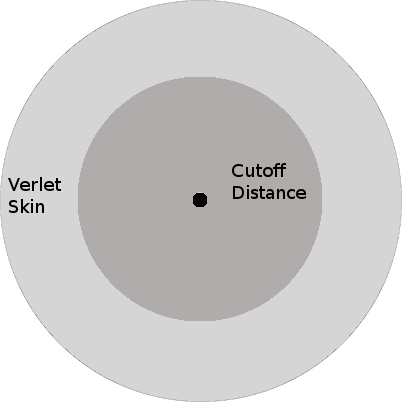
\includegraphics[width=7cm]{Verlet_list.png}
\caption{Verlet skin and cutoff distance for an atom}
\label{fig:verlet_list}
\end{figure}
\subsubsection{Updating the Verlet Lists}
Since updating the Verlet Lists will be a huge time sink for the simulations
(since the update is of complexity $\Theta(N^2)$ the time required will increase
rapidly with an increasing number of atoms). It is therefore necessary to avoid
updating the Verlet Lists unnecessarily often, we have chosen to update the
Verlet Lists only when the total displacement of the two atoms that have moved
the most in the system is greater than the difference between the Verlet Skin
and the cutoff distance of the force calculations.
That is we update if (and only if)
\[
\max_{i=1,\ldots,N}(\texttt{disp}_i) + \max_{i \neq j}(\texttt{disp}_j) \geq
\texttt{Verlet Skin} - \texttt{cutoff}
\]
This way, we update the Verlet Lists only when we might need to (we still update
a few times more than absolutely necessary, but this is hard to avoid).

\subsection{The Verlet Integrator}
In order to integrate the equations of motion for each atom, we need a numerical
integrator. We chose the Velocity Verlet Algorithm for our simulations since it
offers a good pay off between complexity and stability (i.e. time to perform
calculations versus accuracy of calculations). The integration is performed in
two steps. First the new position of each atom is calculated depending on the
velocity and acceleration currently of the atom. In the second step the
new velocity and acceleration of each atom is calculated based on it's new
position as well as it's current and future acceleration (all according to the
Velocity Verlet Algorithm).

Below is the Velocity Verlet algorithm
\begin{equation}
\bar{x}(t + \Delta t) = \bar{x}(t) + \bar{v}(t)\Delta t +
\frac{1}{2}\bar{a}(t)\Delta t^2
\end{equation}
\begin{equation}
\bar{v}(t + \Delta t) = \bar{v}(t) + \frac{\bar{a}(t) + \bar{a}(t+\Delta t)}{2}\Delta t
\end{equation}

\subsubsection{Calculating the Force}
Since (according to Newton) $\bar{F} = m*\bar{a}$ we need the force acting on
each atom in order to get the acceleration of each atom.

In our calculations we use the Lennard-Jones potential
\begin{equation}
V_{LJ} = 4\epsilon\left( \left(\frac{\sigma}{r}\right)^{12} - \left(
\frac{\sigma}{r} \right)^6 \right)
\end{equation}
Where $\epsilon$ and $\sigma$ are material parameters.
And using the fact that 
\begin{equation}
\bar{F} = -\nabla(V)
\end{equation}
We can calculate the force acting on each atom using only it's current position.
In order to save computations we use the fact that $\bar{F}_{ij} = -
\bar{F}_{ji}$ (Newton's third law).

Since we use a truncated Lennard-Jones potential we only calculate the force
between atoms that are within the cutoff distance of each other. Therefore when
we calculate the force on an atom we loop through all atoms in it's Verlet List
and check which of these are within the cutoff distance, instead of looping
through all other atoms in the bulk (or surface).
